\iffalse
\let\negmedspace\undefined
\let\negthickspace\undefined
\documentclass[journal,12pt,twocolumn]{IEEEtran}
\usepackage{cite}
\usepackage{amsmath,amssymb,amsfonts,amsthm}
\usepackage{algorithmic}
\usepackage{graphicx}
\usepackage{textcomp}
\usepackage{xcolor}
\usepackage{txfonts}
\usepackage{listings}
\usepackage{enumitem}
\usepackage{mathtools}
\usepackage{gensymb}
\usepackage{comment}
\usepackage[breaklinks=true]{hyperref}
\usepackage{tkz-euclide} 
\usepackage{listings}
\usepackage{gvv}                                        
\def\inputGnumericTable{}                                 
\usepackage[latin1]{inputenc}                               \usepackage{caption}
\usepackage{color}                                            
\usepackage{array}                                            
\usepackage{longtable}                                       
\usepackage{calc}                                             
\usepackage{multirow}                                         
\usepackage{hhline}                                           
\usepackage{ifthen}                                           
\usepackage{lscape}

\newtheorem{theorem}{Theorem}[section]
\newtheorem{problem}{Problem}
\newtheorem{proposition}{Proposition}[section]
\newtheorem{lemma}{Lemma}[section]
\newtheorem{corollary}[theorem]{Corollary}
\newtheorem{example}{Example}[section]
\newtheorem{definition}[problem]{Definition}
\newcommand{\BEQA}{\begin{eqnarray}}
\newcommand{\EEQA}{\end{eqnarray}}
\newcommand{\define}{\stackrel{\triangle}{=}}
\theoremstyle{remark}
\newtheorem{rem}{Remark}
\begin{document}

\bibliographystyle{IEEEtran}
\vspace{3cm}

\title{NCERT 11.15. Q10}
\author{EE23BTECH11010 - Venkatesh Bandawar$^{*}$% <-this % stops a space
}
\maketitle
\newpage
\bigskip

\renewcommand{\thefigure}{\arabic{figure}}
\renewcommand{\thetable}{\arabic{table}}

\bibliographystyle{IEEEtran}

\parindent 0px
\textbf{Question:} For the travelling harmonic wave
$y\brak {x, t} = 2.0 \cos 2\pi \brak{10t - 0.0080 x + 0.35}$ where $x$ and $y$ are in $cm$ and $t$ in $s$. Calculate the phase difference between oscillatory
motion of two points separated by a distance of 

\begin{enumerate} [label=(\alph*)]
    \item $4 m$
    \item $0.5 m$
    \item $\lambda/2$
    \item $3\lambda/4$
\end{enumerate}

\solution
\fi
\begin{table}[htbp] \small
\centering
\begin{tabular}{|c|c|c|}
	\hline
	\textbf{Symbol} & \textbf{Value} & \textbf{Description} \\[6pt]
	\hline
	$x(0)$ & $25$ & first term of AP \\[6pt]
	\hline
	$d$ & $-3$ & common difference \\[6pt]
	\hline
	$x(n)$ & $(25-3n)u(n)$ & $n$-th term of AP \\[6pt]
	\hline
	$y(n)$ & $116$ & sum of terms \\[6pt]
	\hline 
\end{tabular}

\caption{Given \, parameters list}
\label{tab:11.15.10.1}
\end{table}
\begin{align}
    \brak{\Delta \theta} &= \brak{ 2\pi f t - kx_1 + \phi}  - \brak{2\pi f t -kx_2 + \phi}\\
    &= k\brak{x_2 - x_1} 
\end{align}

\begin{table}[htbp] 
\centering

      \begin{tabular}{|c|c|c|} 
      \hline
\textbf{Variable}& \textbf{Description}& \textbf{Value}\\\hline
         $x(n)$& $n^{th}$ term of sequence& $(2n+1)^2u(n)$\\\hline
          
    \end{tabular}


\caption{Phase \, differences}
\label{tab:11.15.10.2}
\end{table}

\begin{figure}[!h] 
\centering
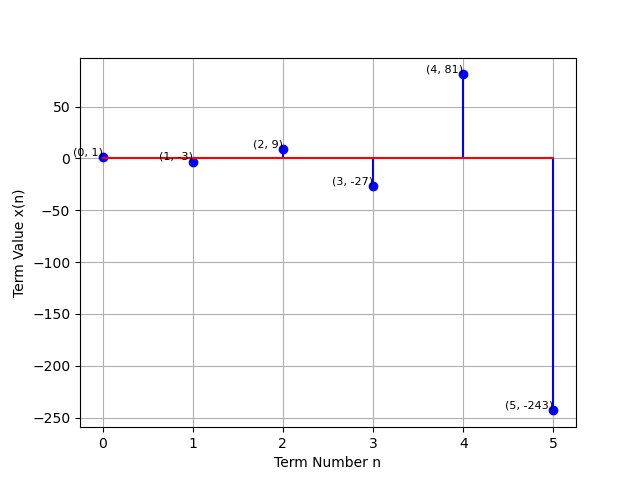
\includegraphics[width=\columnwidth]{ncert-physics/11/15/10/figs/graph1.png}
\captionsetup{justification=centering}
\caption{}
\label{fig:11.15.10.1}
\end{figure}

\begin{figure}[!h] 
\centering
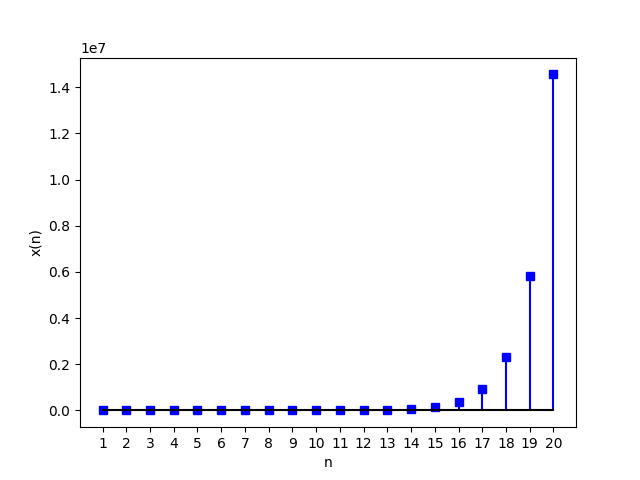
\includegraphics[width=\columnwidth]{ncert-physics/11/15/10/figs/graph2.png}
\captionsetup{justification=centering}
\caption{}
\label{fig:11.15.10.2}
\end{figure}

\begin{figure}[!h] 
\centering
\includegraphics[width=\columnwidth]{ncert-physics/11/15/10/figs/graph3.png}
\captionsetup{justification=centering}
\caption{}
\label{fig:11.15.10.3}
\end{figure}

\begin{figure}[!h] 
\centering
\includegraphics[width=\columnwidth]{ncert-physics/11/15/10/figs/graph4.png}
\captionsetup{justification=centering}
\caption{}
\label{fig:11.15.10.4}
\end{figure}

